\chapter{Results, Reproducibility, and Evaluation Status}
\label{ch:results}

\section{Purpose of this chapter}
This chapter distinguishes executable evidence from legacy illustrative material. Performance values are reported only when they are generated by the repository's evaluation script and accompanied by a split-integrity assessment. This distinction is essential because an image-level split can produce optimistic estimates when scans or views from the same subject occur in more than one partition.

\section{Current cohort audit}
The supplied directories contain 402 training, 107 validation, and 120 test images when the configured combined loader is used. The audit script reports that subject \texttt{30nh} appears in both OASBUD training and validation data, while BrEaST cases \texttt{case140} and \texttt{case151} span partitions. In addition, the BUSI copy uses generated \texttt{sample\_} filenames, preventing verification of patient-level separation from the local files alone. The current cohort consequently does not support a patient-independent performance claim.

\section{Executable checkpoint result}
The included EfficientNet-B0 checkpoint was evaluated with the shared preprocessing implementation on the current test partition. Table~\ref{tab:provisional_result} is generated from that execution and is retained as a software-regression reference, not as a clinical or generalisation result.

\begin{table}[htbp]
\centering
\caption{Provisional result from the bundled EfficientNet-B0 checkpoint on the unaudited 120-image test partition.}
\label{tab:provisional_result}
\begin{tabular}{@{}lccccc@{}}
\toprule
\textbf{Model} & \textbf{Samples} & \textbf{Accuracy} & \textbf{Macro F1} & \textbf{Macro Recall} & \textbf{ROC-AUC} \\ \midrule
EfficientNet-B0 & 120 & 78.33\% & 0.7811 & 0.7809 & 0.8612 \\ \bottomrule
\end{tabular}
\end{table}

At class level, the benign class (62 images) had precision 0.76, recall 0.85, and F1 0.80. The malignant class (58 images) had precision 0.82, recall 0.71, and F1 0.76. These values confirm that the checkpoint, data loader, and evaluator run together; they do not resolve the cohort-leakage issue.

The confusion matrix in Figure~\ref{fig:provisional_confusion} contains 53 correctly classified benign images, 41 correctly classified malignant images, 9 benign images classified as malignant, and 17 malignant images classified as benign. Figure~\ref{fig:provisional_roc} plots the corresponding threshold sweep. Both figures are generated by \texttt{evaluate.py} from the same prediction run as Table~\ref{tab:provisional_result}.

\begin{figure}[htbp]
    \centering
    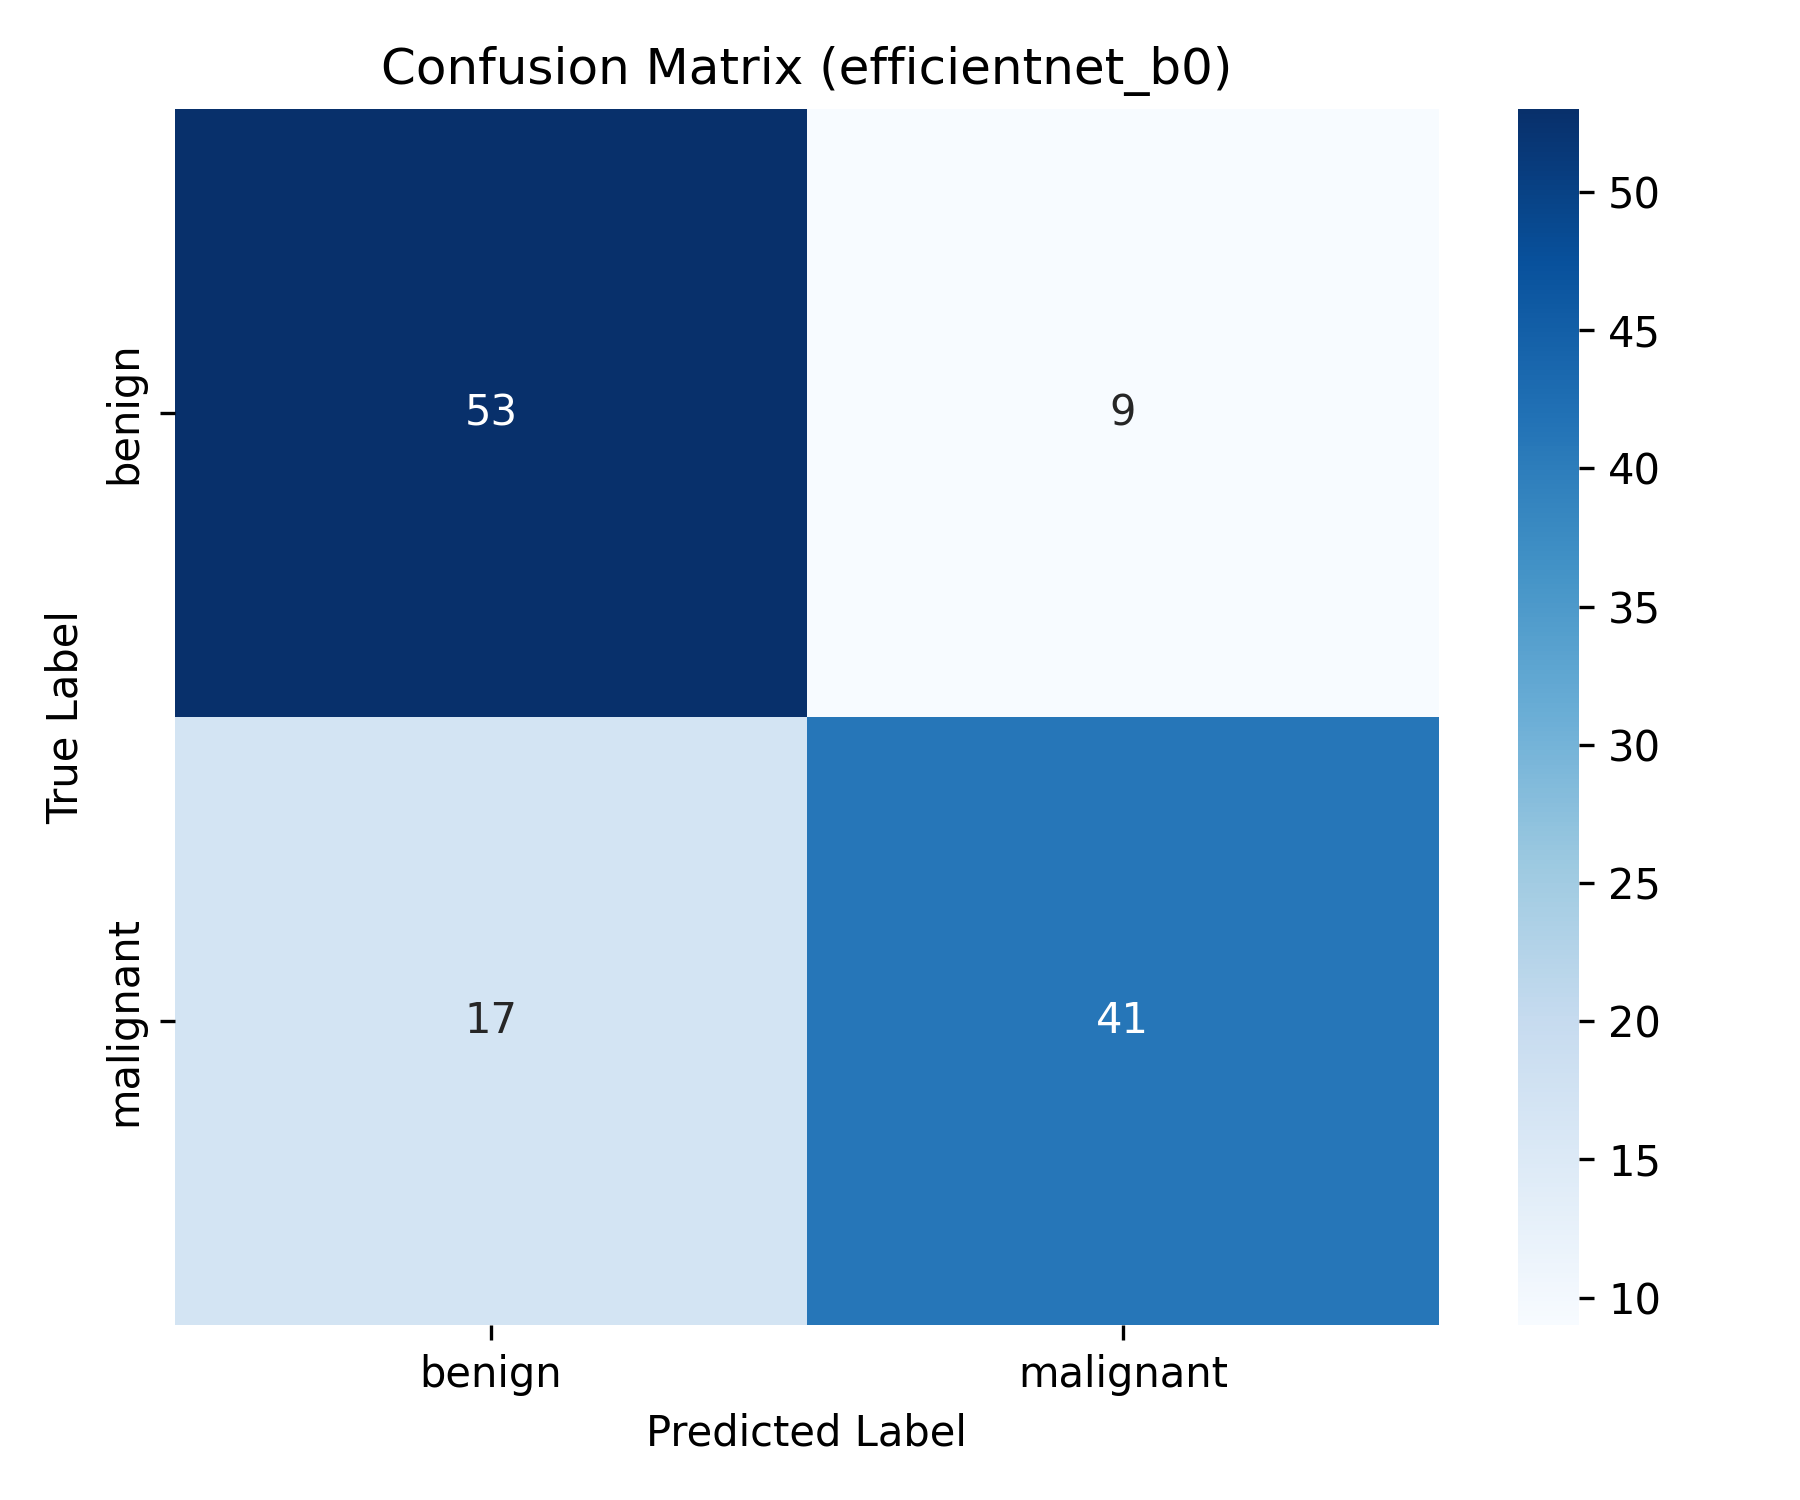
\includegraphics[width=0.72\textwidth]{figures/fig2_confusion_matrix.png}
    \caption{Confusion matrix for the bundled EfficientNet-B0 checkpoint on the current unaudited test folders. Provisional engineering evidence only.}
    \label{fig:provisional_confusion}
\end{figure}

\begin{figure}[htbp]
    \centering
    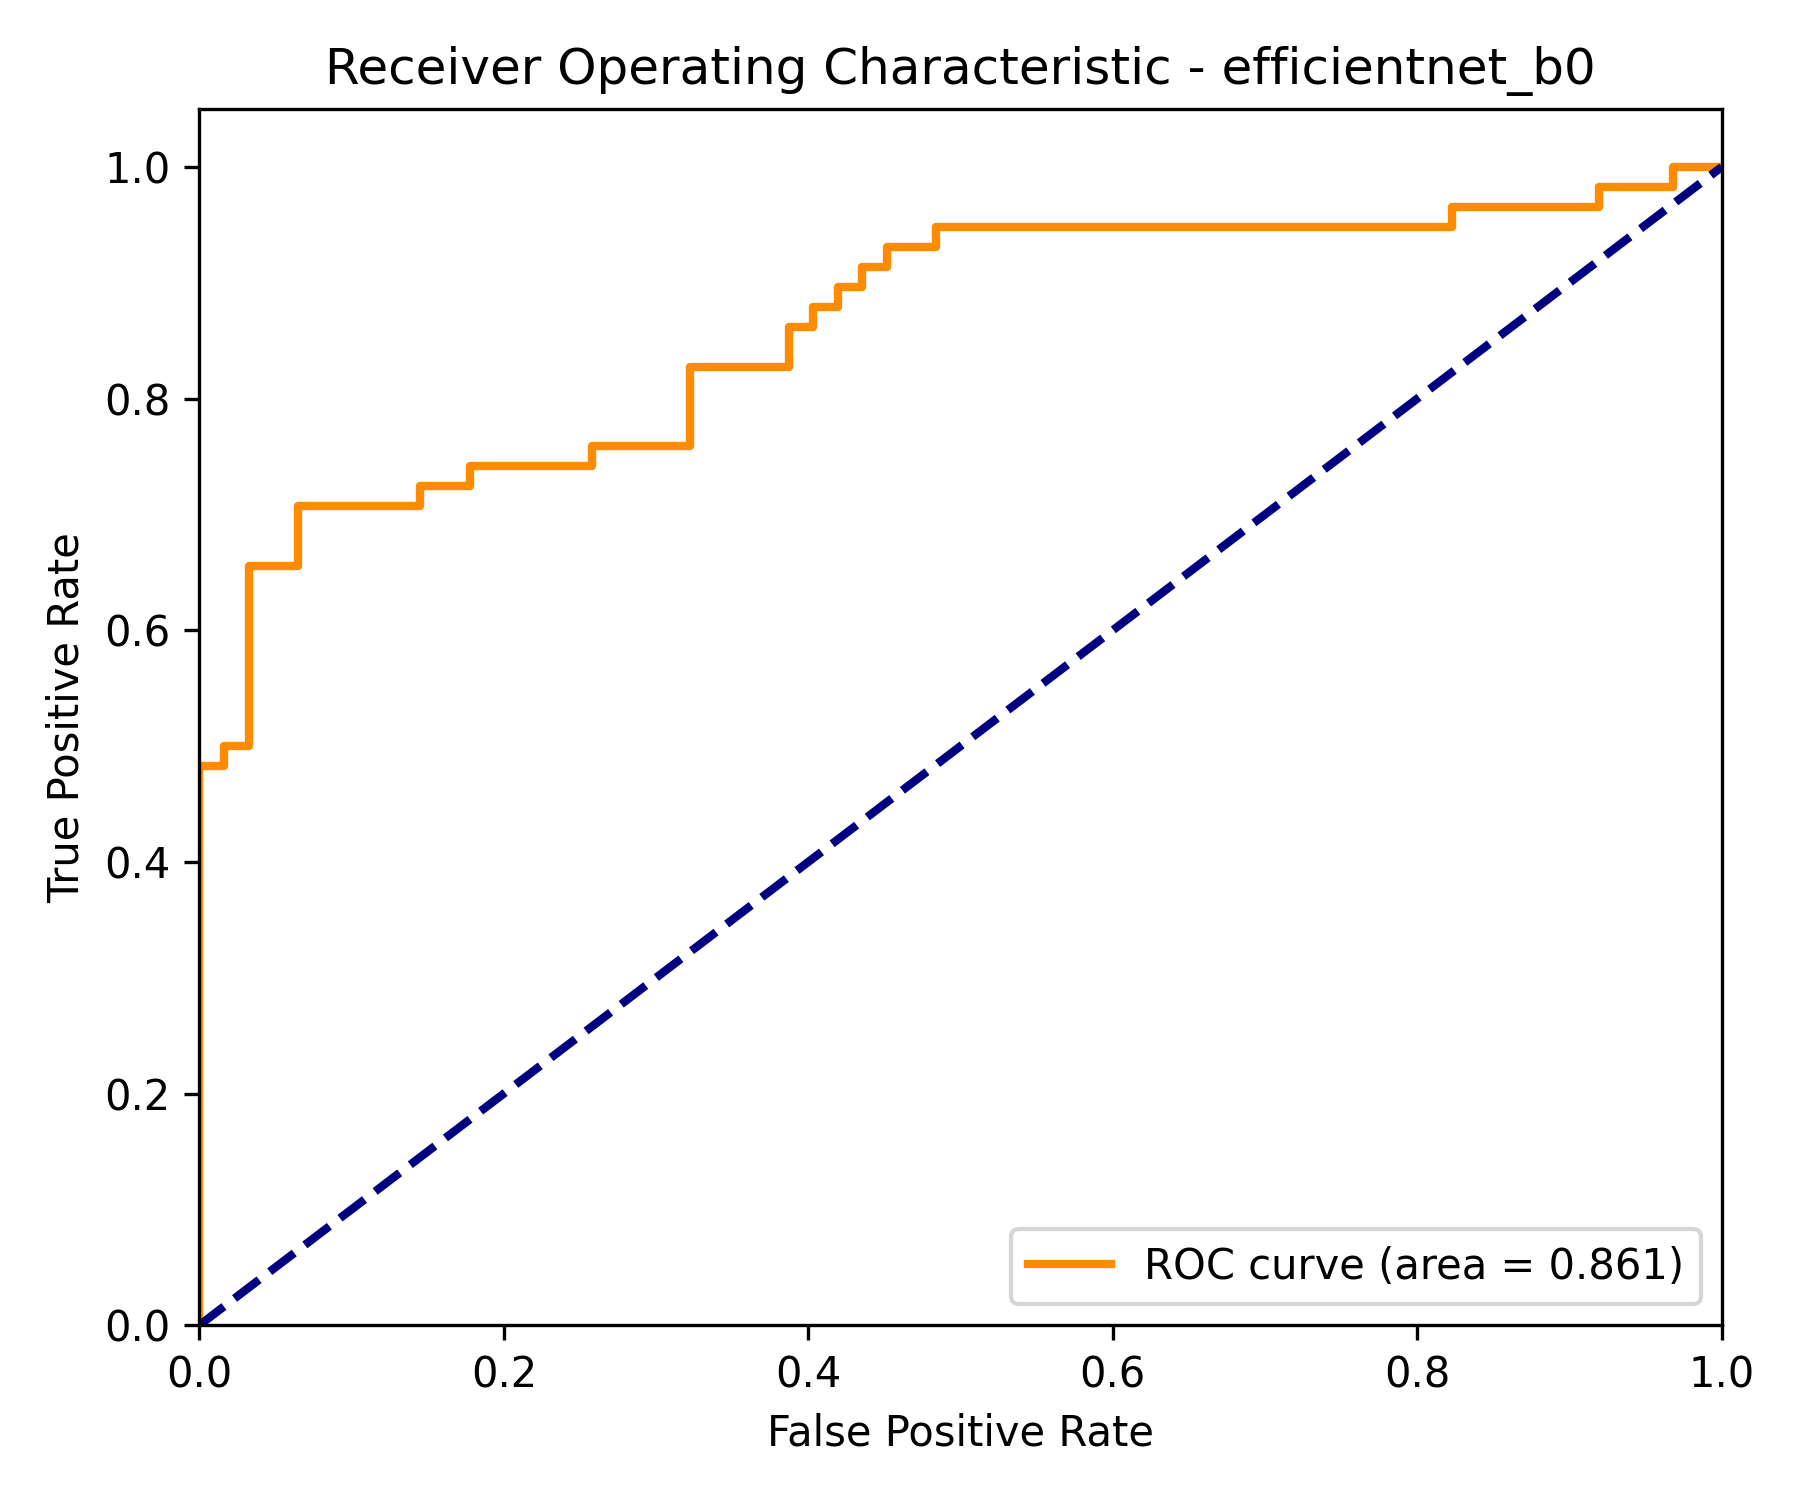
\includegraphics[width=0.72\textwidth]{figures/fig3_roc_curve.png}
    \caption{ROC curve for the same provisional 120-image evaluation run (ROC-AUC 0.8612).}
    \label{fig:provisional_roc}
\end{figure}

\section{Withdrawn legacy figures and tables}
Earlier project assets contained fixed benchmark values, simulated pseudo-labelling tables, and illustrative noise trajectories. They are not used as results because they were not regenerated from stored model predictions on an audited cohort. The superseded files have been removed from the submission-facing figures and archived with an explicit warning; they must not be cited as measured performance.

\section{Final evaluation protocol}
The final study must assign every subject, including all views and masks, to exactly one partition. It should preserve a versioned manifest with source identifiers, label, split, checksum, preprocessing configuration, random seed, checkpoint hash, and per-image prediction. Accuracy, sensitivity, specificity, ROC-AUC, precision--recall AUC, calibration, and confidence intervals should then be calculated once on an untouched test partition. Noise and preprocessing ablations require separate trained/evaluated runs rather than manually specified curves.

\section{Interpretation}
The present evidence supports the implementation of a reproducible experimental framework, not superiority of a particular architecture or preprocessing method. The results should therefore be interpreted as a baseline engineering validation. Claims of clinical robustness, optimal pseudo-labelling thresholds, or state-of-the-art diagnostic performance are deferred pending the audited experiments described above.
